\documentclass{article}
\usepackage[margin=3cm]{geometry}
\usepackage[utf8]{inputenc}
\usepackage{float}
\usepackage{graphicx} % Required for figures
\usepackage{anysize}
\usepackage{booktabs}
\usepackage{hyperref}

\title{\bfseries\Huge CV}
%\author{Thomas Krogh Lohse}
\date{}
\begin{document}
\section*{\Huge CV}


\begin{minipage}{0.76\textwidth}
    \begin{tabular}{ll}
        \toprule%\\[-10pt]
        \textbf{Name:} Thomas Krogh Lohse                 
            & \textbf{Github:} \href{https://github.com/LohseBoi}{@LohseBoi} \\[2pt]
        \textbf{Address:} Thulevej 8 3th, Aalborg SØ 9210 
            & \textbf{Gitlab:} \href{https://gitlab.com/LohseBoi}{@LohseBoi} \\[2pt]
        \textbf{Private E-mail:} \href{mailto:thomas.k.lohse@gmail.com}{thomas.k.lohse@gmail.com} 
            & \textbf{Phone:} +45 51 16 41 99 \\[2pt]
        \textbf{School E-mail:} \href{mailto:tlohse20@student.aau.dk}{tlohse20@student.aau.dk}   
            & \textbf{Subject:} gamer \\[2pt]
        \textbf{Educational Level:} High School (Level 4) & \textbf{Subject:} gamer \\%[2pt]
        \bottomrule
    \end{tabular}
\end{minipage}
\begin{minipage}{0.2\textwidth}
    \flushright{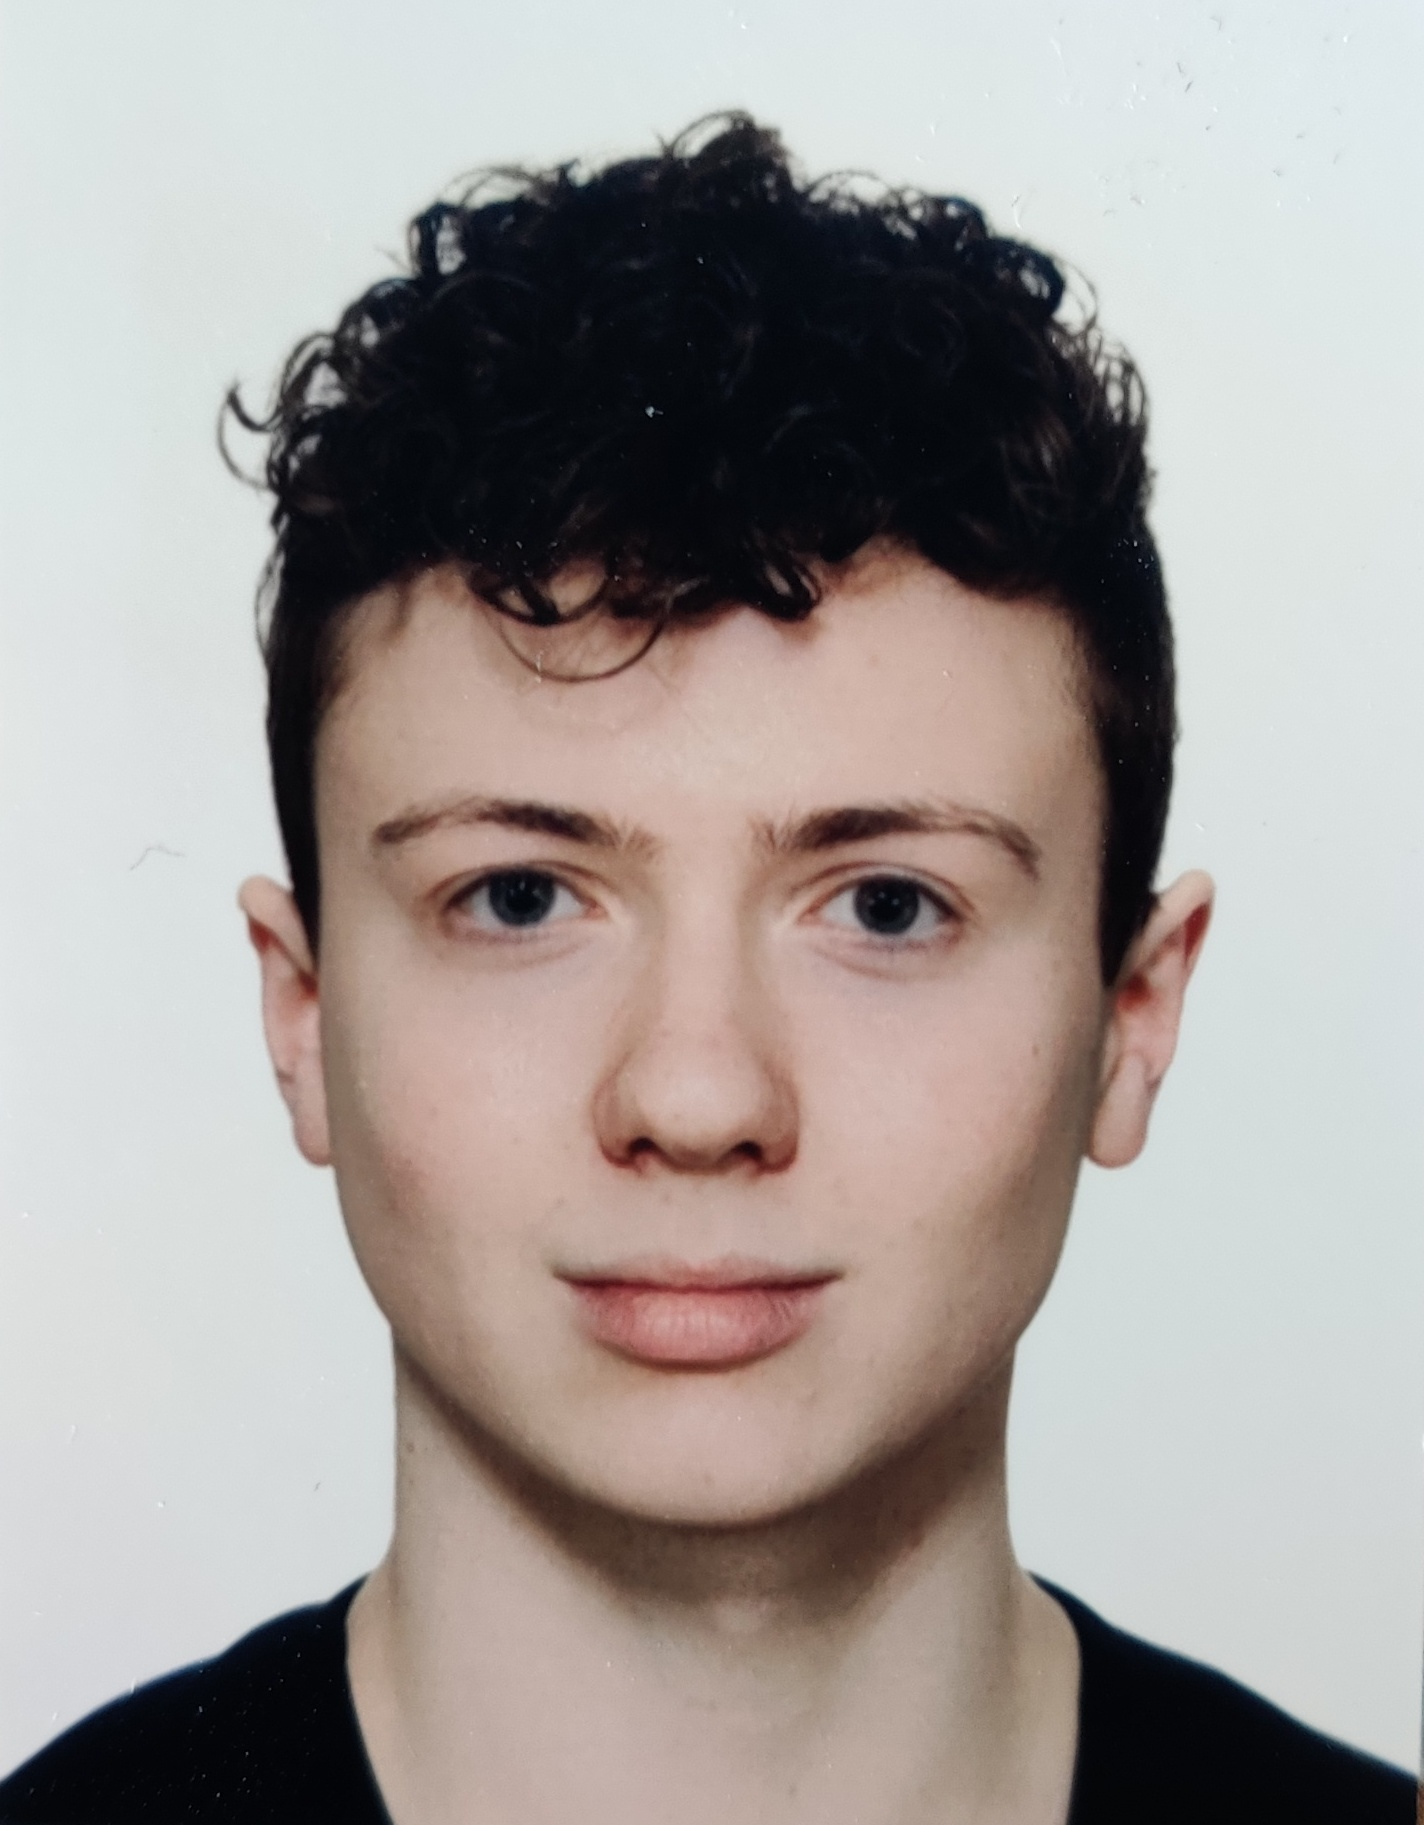
\includegraphics[width=3cm]{./Portrait.jpg}}
\end{minipage}
\\
    \section*{Education}
    %\lipsum[4]\\[0.5cm]
    \begin{tabular}{r|p{.82\linewidth}} %TODO
        2007 -- 2016 & \textbf{Public School}\\
    &   blablabla
        \\\\
        2016 -- 2017 & \textbf{Efterskole (Boarding School)}\\
    &   blablabla
        \\\\
        2017 -- 2020 & \textbf{High School}\\
    &   blablabla
        \\\\
        2019 & \textbf{Van Driver Training Certificate }\\
    &   blablabla
        \\\\
        2020 -- Now & \textbf{University}\\
    &   blablabla
    \end{tabular}
 
    \section*{Employment \& Other Experience}
    \subsection*{Employment}
    \begin{tabular}{r|p{.82\linewidth}}%TODO
        2014 -- 2016 & \textbf{Advertisment Magazine Distributor}\\
    &   blablabla
        \\\\
        2018 -- 2019 & \textbf{Føtex Nørresundby}\\
    &   blablabla
    \end{tabular}

    \subsection*{Other}
    \begin{tabular}{r|p{.82\linewidth}}
        2021 -- Now & \textbf{UNF Game Development Camp}\\
    &   I am a volunteer at UNFs Game Development Camp, where I have had the following roles:
        \begin{itemize}\setlength\itemsep{0em}
            \item[2021] \textbf{Programmings Assistant ---} Assisting the programming teacher, and
                helping the campers with any programming related issues they might have.
            \item[2021] \textbf{Logistics Responsible ---} In charge of handling the logistical
                requests of the other volunteers, and acquiring said logistics.
            \item[2022] \textbf{Technical Manager ---} In charge of making sure the campers'
                equipment is operational, along with introducing \verb|git|, and managing the
                problems they might have with them.
        \end{itemize}
        \\
        2021 & \textbf{Tutor}\\
    &   I volunteered as a tutor for the students in 2021, studying Software at Aalborg University. 
    \end{tabular}

    \section*{Sparetime Hobbies/Activities}
    \begin{itemize}\setlength\itemsep{0.5em}
        \item[] \textbf{Physical Activity}\\
            I make sure to stay ohysically active, mainly in the form of strengh training in the
            gym.
        \item[] \textbf{IT-Tinkering}\\
            By IT-tinkering, I refer to my own programming projects/exercises, along with tinkering
            with my Linux-system on my laptop and the firmware on my self-build keyboard.
        \item[] \textbf{Programming youth club}\\
            On tuesdays I attend a programming youth club called GameLab, which is managed by
            UngAalborg.
        \item[] \textbf{Gaming}\\
            blablabla %TODO
    \end{itemize}

    \section*{References}
    \begin{tabular}{r|p{.82\linewidth}}
        Føtex Nørresundby & \textbf{Sabine Them}                                    \\
        &Tlf.: +45 22 46 98 93                                                      \\
        &E-mail: \href{mailto:sabine.them@foetex.dk}{sabine.them@foetex.dk}         \\[.3cm]
        Føtex Nørresundby & \textbf{Joan Jørgensen}                                 \\
        &Tlf.: +45 22 72 06 61                                                      \\
        &E-mail: \href{mailto:joan.joergensen@foetex.dk}{joan.joergensen@foetex.dk} \\[.3cm]
        GameLab UngAalborg & \textbf{Christian "Code" Skriver Kragegaard}           \\
        &Tlf.: +45 93 52 09 10                                                      \\
        &E-mail: \href{mailto:Csk-skole@ungaucnet.dk}{Csk-skole@ungaucnet.dk}       \\
    \end{tabular}

\end{document}

\iffalse%
    \lipsum[4]\\[0.5cm]
    \begin{tabular}{r|p{.82\linewidth}}
        Start -- End: & \textbf{Occupation}\\
    &   blablabla
        \\\\
        Start--End: & \textit{Occupation}\\
    &   blablabla
        \\\\
        \textbf{Start -- End:} & \textbf{Occupation}\\
    &   blablabla
        \\\\
        \textbf{Start--End:} & \textit{Occupation}\\
    &   blablabla
    \end{tabular}
\fi

\iffalse&
\begin{tabularx}{\linewidth}{llr}
    \toprule%\\[-10pt]
    \textbf{Name:} Thomas Krogh Lohse                 
        & \textbf{Github:} \href{https://github.com/LohseBoi}{@LohseBoi}
        & \multirow{3}{*}{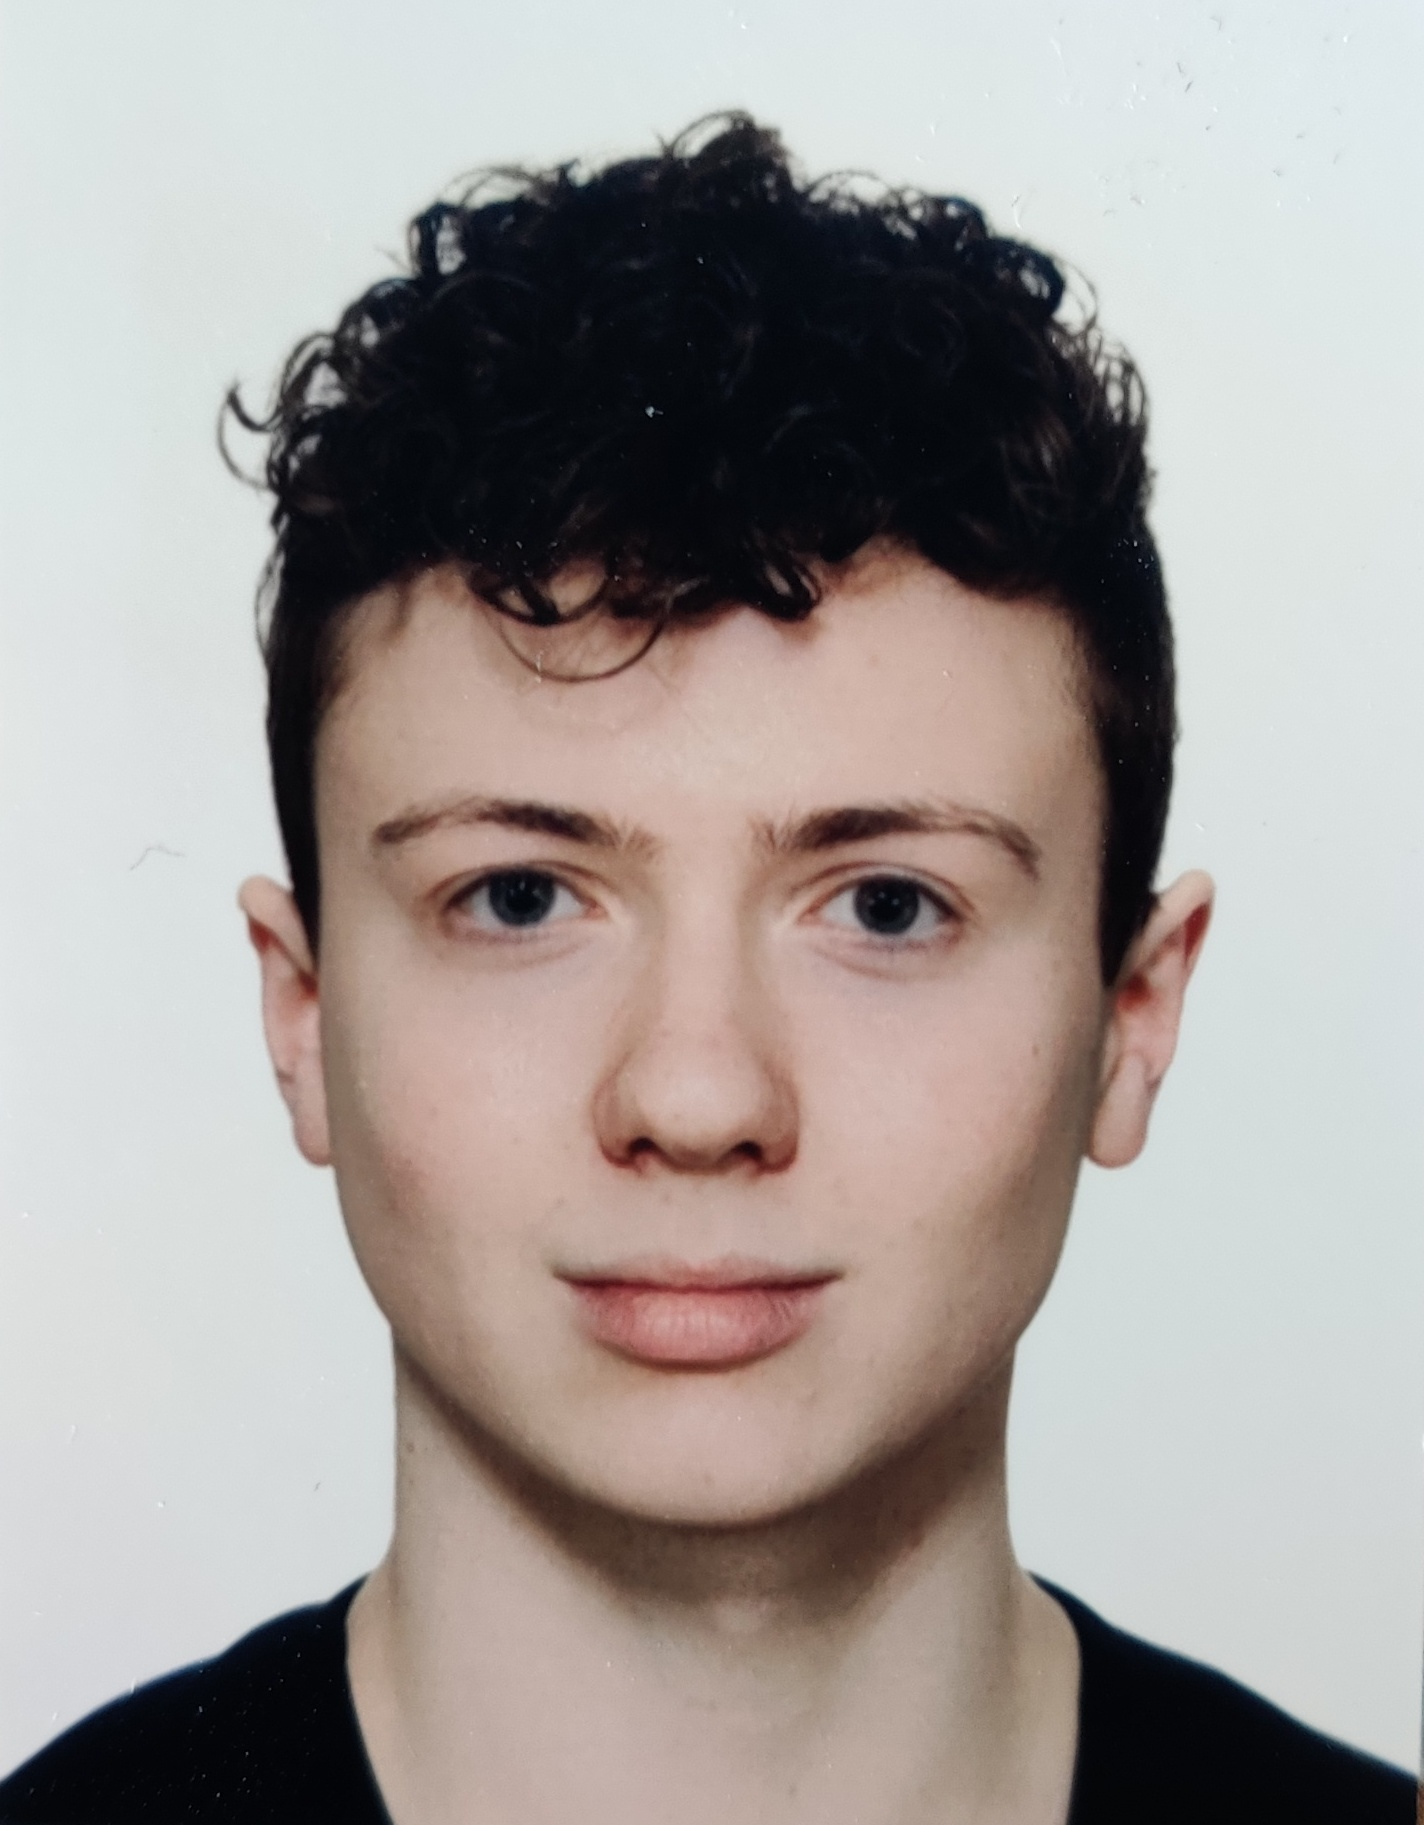
\includegraphics[width=1.85cm]{./Portrait.jpg}}\\[2pt]
    \textbf{Address:} Thulevej 8 3th, Aalborg SØ 9210 
        & \textbf{Gitlab:} \href{https://gitlab.com/LohseBoi}{@LohseBoi} \\[2pt]
    \textbf{Private E-mail:} \href{mailto:thomas.k.lohse@gmail.com}{thomas.k.lohse@gmail.com} 
        & \textbf{Phone:} +45 51 16 41 99 \\[2pt]
    \textbf{School E-mail:} \href{mailto:tlohse20@student.aau.dk}{tlohse20@student.aau.dk}   
        & \textbf{Subject:} gamer \\[2pt]
    \textbf{Educational Level:} High School (Level 4) & \textbf{Subject:} gamer \\%[2pt]
    \bottomrule
\end{tabularx}
\fi

